% !TeX spellcheck = ru_RU
% !TEX root = vkr.tex

\label{sec:relatedworks}

\subsection{Обзор аналогичных инструментов}
Выбор в пользу библиотеки Brahma.FSharp для использования в описанном выше прототипе был обусловлен рядом причин. При поиске инструмента для взаимодействия с GPGPU критериями отбора являлись перечисленные ниже параметры.
% В обзоре были рассмотрены интересующие аспекты некоторых аналогичных инструментов для работы с GPGPU. Критерием отбора являлось наличие у инструмента одного из следующих параметров:
\begin{itemize}
    \item \textbf{Возможность описывать ядра для GPGPU на языке высокого уровня.} Такая возможность может позволить достичь уровня переносимости, необходимого в задачах обобщенной линейной алгебры. Многие библиотеки, представляющие собой высокоуровневые обертки над вызовами к API GPU, такие как pyopencl\footnote{Репозиторий библиотеки pyopencl: \url{https://github.com/inducer/pyopencl}. Дата обращения: 17.03.2022}, pycuda\footnote{Репозиторий библиотеки pyopencl: \url{https://github.com/inducer/pycuda}. Дата обращения: 17.03.2022}, OpenCL.NET\footnote{Репозиторий библиотеки OpenCL.NET: \url{https://github.com/dgsantana/OpenCL.NET}. Дата посещения: 01.06.2021}, Cloo\footnote{Репозиторий библиотеки Cloo: \url{https://github.com/clSharp/Cloo}. Дата посещения: 01.06.2021}, JavaCL\footnote{Репозиторий библиотеки JavaCL: \url{https://github.com/nativelibs4java/JavaCL}. Дата посещения: 01.06.2021}, JOCL\footnote{Репозиторий библиотеки JOCL: \url{https://github.com/gpu/JOCL}. Дата посещения: 01.06.2021} и другие, не удовлетворяют этому критерию и не подходят для использования в описанном контексте.
    \item \textbf{Использование OpenCL в качестве платформы исполнения.} Решения, основанные на платформе OpenCL, более переносимы, чем аналогичные решения для других платформ, таких как NVIDIA CUDA и Metal. По этой причине из рассмотрения были исключены некоторые инструменты, такие как, например, Numba\footnote{Репозиторий библиотеки Numba: \url{https://github.com/numba/numba}. Дата посещения: 09.03.2022}.
    \item \textbf{Возможность описывать собственные ядра.} Такая возможность является необходимой для реализации многих алгоритмов, требуемых в библиотеке обобщенной разреженной линейной алгебры. По причине несоответствия этому критерию из рассмотрения была исключена, например, библиотека Accelerate\footnote{Репозиторий библиотеки Accelerate: \url{https://github.com/AccelerateHS/accelerate}. Дата посещения: 09.03.2022}.
    \item \textbf{Возможность использовать данные произвольных (или почти произвольных) типов, в том числе обобщенных.} Такая возможность необходима, так как стандарт GraphBLAS не накладывает ограничения на используемые типы данных. По этому критерию были исключены из рассмотрения такие библиотеки, как Aparapi\footnote{Репозиторий библиотеки Aparapi: \url{https://github.com/aparapi/aparapi}. Дата посещения: 09.03.2022} и SPOC\footnote{Репозиторий библиотеки SPOC: \url{https://github.com/mathiasbourgoin/SPOC}. Дата обращения: 09.03.2022}.
    \item \textbf{Возможность использования на платформе .NET или Java.} Эти платформы достаточно популярны, чтобы потенциальный инструмент для обобщенной линейной алгебры был более востребован.
    \item \textbf{Инструмент написан на функциональном языке программирования.} Для функциональных языков программирования могут быть доступны некоторые техники суперкомпиляции и оптимизации, например kernel fusion~\cite{fusion} и deforestation~\cite{deforset}, которые могли бы улучшить производительность разрабатываемого инструмента. По причине несоответствия этому критерию из рассмотрения были исключены, например, библиотеки ILGPU\footnote{Репозиторий библиотеки ILGPU: \url{https://github.com/m4rs-mt/ILGPU}. Дата посещения: 09.03.2022} и Alea GPU.
\end{itemize} 

В конечном итоге среди инструментов, подходящих под заданные требования, остались FSCL\footnote{Репозиторий библиотеки FSCL: \url{https://github.com/FSCL/FSCL.Runtime}. Дата посещения: 09.03.2022} --- библиотека для языка программирования F\#, позволяющая работать с OpenCL, и библиотека Brahma.FSharp. Библиотека FSCL, несмотря на преимущества в виде продвинутой поддержки исполнения программ в multi-GPU режиме, оказалось недостаточно гибкой из-за особенной модели программирования. К тому же, библиотека давно не поддерживается. По этой причине была выбрана библиотека Brahma.FSharp, разрабатывающаяся на кафедре системного программирования СПбГУ.

\subsection{Платформа OpenCL и модель исполнения}
% % \subsubsection{}
% OpenCL --- это фреймворк для написания параллельных программ, способных исполняться на множестве гетерогенных платформ.
Центральным элементом платформы OpenCL~\cite{ocl} является понятие хоста --- устройства, которое координирует вычисления и осуществляет взаимодействие с пользователем. Команды, переданные с хоста, выполняются на OpenCL устройствах, которые могут быть представлены во множественном числе и отличаться по типу (CPU, GPU, FPGA) и платформе (AMD, Intel и так далее). OpenCL устройства логически делятся на вычислительные модули (compute units), которые в свою очередь делятся на обрабатывающие элементы (processing elements). Схематическое изображение модели платформы показано на рисунке~\ref{fig:opencl_pl}.
Между хостом и OpenCL устройствами существуют отличия в том числе в модели программирования. OpenCL программа, по сути, состоит из двух частей --- кода ядер, которые реализуют параллельные вычисления и запускаются на OpenCL устройствах, и программы хоста, которая управляет ресурсами устройств, координирует исполнение OpenCL ядер и так далее.

Взаимодействие между хостом и OpenCL устройством происходит посредством команд, помещенных в очередь команд (command queue). Хост отправляет команды в очередь, после чего они устанавливаются планировщиком для исполнения на устройствах. Команды могут отвечать за выполнение ядер, управление памятью и синхронизацию выполнения команд в очереди. Они исполняются асинхронно между хостом и устройством. Команды могут выполняться последовательно (in-order execution) или внеочередно (out-of-order execution). Координация команд исполнения ядер и команд управления памятью может быть осуществленна в том числе за счет объектов-событий, которые генерируют эти команды.

\begin{figure}[h!]
\centering
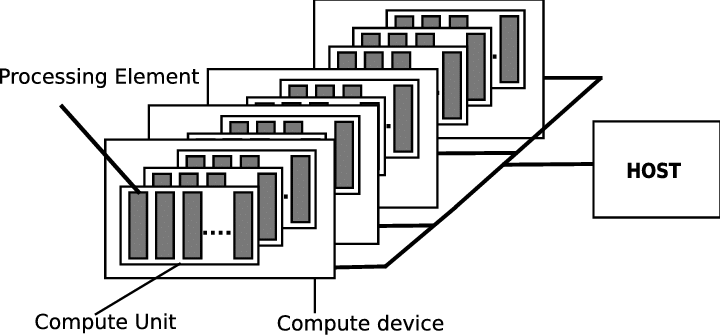
\includegraphics[scale=0.4]{pictures/OpenCL-Host-Device-Architecture.png}
\caption{Архитектура платформы OpenCL~\cite{opencl_pl}}
\label{fig:opencl_pl}
\end{figure}

Кроме того, OpenCL определяет индексное пространство (NDRange), которое может иметь от 1 до 3 измерений. Индексное пространство содержит множество точек, называемых рабочими элементами (work-items). Каждый рабочий элемент имеет уникальный индекс в глобальном индексном пространстве и занимается параллельным исполнением ядра, код которого является общим для всех элементов. Рабочие элементы ко всему прочему сгруппированы в рабочие группы (work-groups) заранее определенного размера. Соответственно, рабочий элемент обладает также локальным индексом --- уникальным идентификатором внутри рабочей группы. Элементы внутри одной рабочей группы могут синхронизироваться, а также имеют доступ к общей локальной памяти.  Схематическое изображение индексного пространства показано на рисунке~\ref{fig:opencl_sp}.

\begin{figure}[h!]
\centering
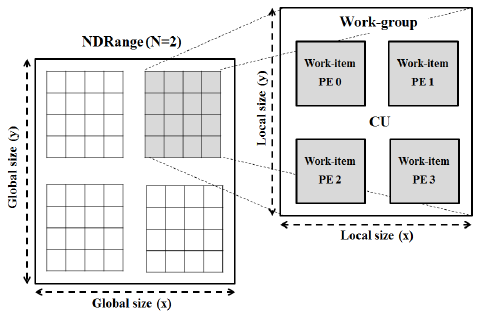
\includegraphics[scale=0.45]{pictures/The-index-space-of-OpenCL.png}
\caption{Модель индексного пространства OpenCL~\cite{ocl_sp}}
\label{fig:opencl_sp}
\end{figure}

% \subsubsection{Ресурсы и контекст OpenCL}
% Программа хоста определяет контекст выполнения OpenCL и управляет следующими ресурсами:
% \begin{itemize}
%     \item \textbf{Устройства} --- набор OpenCL устройств, используемых хостом для запуска ядер;
%     \item \textbf{Ядра} --- набор исполняемых OpenCL вычислений;
%     \item \textbf{Программы} --- набор скомпилированных из исходного кода ядер программ;
%     \item \textbf{Память} --- набор объектов содержащих данные, которые доступны для чтения и записи как программой хоста, так и ядром.
%     \item \textbf{Очередь команд} --- 
% \end{itemize}

\subsection{Язык программирования F\#}
F\# --- это мультипарадигменный язык программирования из семейства языков платформы .NET. Язык позволяет писать типобезопасные программы в функциональном стиле благодаря строгой типизации и поддержке функциональной парадигмы. Среди характеристик языка можно выделить особенности, описанные ниже.
\begin{itemize}
    \item \textbf{Размеченные объединения.} Размеченное объединение является типом, представляющим собой конечный набор альтернатив. Примером размеченного объединения является тип \verb|Option|, имеющий 2 альтернативы: \verb|Some| --- наличие значения, и \verb|None| --- его отсутствие. 
    \item \textbf{Цитирование (F\# Quotations).} Механизм цитирования позволяет представить блок кода на языке F\# в виде абстрактного синтаксического дерева. Благодаря этому программист может проводить анализ и преобразование такого дерева во время исполнения. Среди доступных применений этой особенности стоит выделить возможность преобразовывать код на языке программирования F\# в код на другом языке. Для того чтобы создать цитату выражения языка F\#, его нужно обернуть в специальные кавычки \verb|<@ ... @>|. Выражение, объявленное таким образом, компилируется в значение типа \verb|Quotations.Expr|, представляющее собой абстрактное синтаксическое дерево этого выражения.
    \item \textbf{Вычислительные выражения.} Вычислительные выражения представляют собой особый механизм описания вычислений. С их помощью могут быть описаны, например, монады, моноиды, апликативыне функторы. С их помощью можно описывать недетерминированные вычисления, асинхронные вычисления, вычисления с побочными эффектами. 
\end{itemize}

\subsection{Библиотека Brahma.FSharp}
Brahma.FSharp --- это библиотека, которая позволяет использовать возможности OpenCL в проектах на языке F\#.
Её особенности перечислены ниже.
\begin{itemize}
    \item Позволяет использовать подмножество языка F\# для написания кода ядер OpenCL.
    \item Позволяет проверять некоторые ошибки на этапе компиляции.
    \item Поддерживает трансляцию пользовательских типов данных.
    \item Обеспечивает переносимость за счет кодогенерации.
\end{itemize}

\noindent Библиотека состоит из двух основных компонентов:
\begin{itemize}
    \item транслятора из F\# в OpenCL;
    \item API хоста для запуска ядер и управления памятью.
\end{itemize}

\subsubsection{Описание OpenCL ядер}
Для описания ядер OpenCL используется механизм цитирования F\# кода. Ядро описывается лямбда-функцией с типом \verb|#NDRange -> 'a|, где первым аргументом передаются данные об индексном пространстве ядра. При этом ядро может быть полиморфно относительно типа данных, с которыми оно работает. Внутри ядра возможно использовать почти любые выражения языка F\#, а также некоторые специально определенные функции из библиотеки Brahma.FSharp. К таким функциям относятся, например: \verb|barrierLocal()| для создания синхронизирующего барьера внутри рабочей группы или \verb|localArray<'a>| для выделения локальной памяти. Пример описания простейшего ядра приведен в листинге~\ref{lst:ex}.

\newpage

% \begin{lstlisting}[caption=Пример описания простейшего ядра на языке F\#, language=Caml, frame=single, label={lst:ex}]
% let kernel =
%     <@
%         fun (range: Range1D) (buffer: 'a clarray) (value: 'a) ->
%             let gid = range.GlobalID0
%             buffer.[gid] <- value
%     @>
% \end{lstlisting}

\subsubsection{Транслятор}
В библиотеке используется машинно-зависимый транслятор, состоящий из трёх частей:
\begin{itemize}
    \item модуля, который занимается преобразованием абстрактного синтаксического дерева кода на F\#;
    \item модуля, который преобразует абстрактное синтаксическое дерево кода на F\# в дерево языка ядер OpenCL;
    \item модуля, который по дереву языка ядер OpenCL генерирует OpenCL код. 
\end{itemize}

Модель трансляции изображена на рисунке~\ref{fig:transl}.
\begin{figure}[!h]
\centering
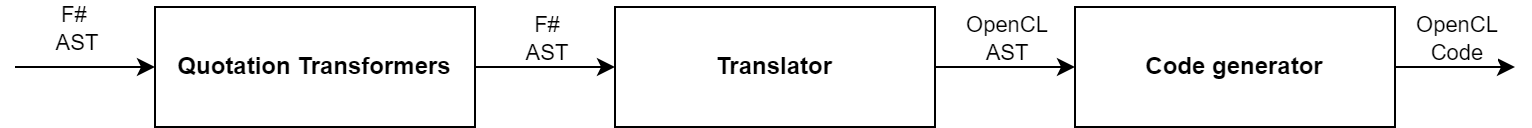
\includegraphics[scale=0.3]{pictures/Translator.png}
\caption{Модель трансляции, используемая в библиотеке Brahma.FSharp}
\label{fig:transl}
\end{figure}

Среди его особенностей можно выделить следующие:
\begin{itemize}
    \item поддерживает возможность использования вложенных функций;
    \item поддерживает возможность печати в консоль изнутри ядра;
    \item поддерживает возможность использования в коде ядра пользовательских типов данных. 
\end{itemize}

\begin{lstlisting}[caption=Пример описания простейшего ядра на языке F\#, language=Caml, frame=single, label={lst:ex}]
let kernel =
    <@
        fun (range: Range1D) (buffer: 'a clarray) (value: 'a) ->
            let gid = range.GlobalID0
            buffer.[gid] $\leftarrow$ value
    @>
\end{lstlisting}


% % возможность описывать ядра CUDA/OpenCL на языке высокого уровня, наличие поддержки OpenCL, возможность использования инструмента на платформе .NET, инструмент написан на функциональном языке программирования, наличие открытого исходного кода. 
% Отобранные инструменты перечислены в таблице~\ref{tab:gpgpu}.

% \begin{table}
%     % \centering
%     \begin{minipage}{\linewidth}
%     \begin{tabularx}{\textwidth}{X|X|X}
%     Инструмент & Язык & Платформа \\
%     \hline
%     Numba\footnote{Репозиторий библиотеки Numba: \url{https://github.com/numba/numba}. Дата посещения: 09.03.2022} & Python & CUDA \\
%     Aparapi\footnote{Репозиторий библиотеки Aparapi: \url{https://github.com/aparapi/aparapi}. Дата посещения: 09.03.2022} & Java & OpenCL \\
%     ILGPU\footnote{Репозиторий библиотеки ILGPU: \url{https://github.com/m4rs-mt/ILGPU}. Дата посещения: 09.03.2022} & .NET & CUDA/OpenCL \\
%     FSCL\footnote{Репозиторий библиотеки FSCL: \url{https://github.com/FSCL/FSCL.Runtime}. Дата посещения: 09.03.2022} & F\# & OpenCL \\
%     Accelerate\footnote{Репозиторий библиотеки Accelerate: \url{https://github.com/AccelerateHS/accelerate}. Дата посещения: 09.03.2022} & Haskell & CUDA \\
%     SPOC\footnote{Репозиторий библиотеки SPOC: \url{https://github.com/mathiasbourgoin/SPOC}. Дата обращения: 09.03.2022} & OCaml & CUDA/OpenCL \\
%     \hline
%   \end{tabularx}
%   \end{minipage}
%   \caption{Инструменты, участвовавшие в обзоре}
%   \label{tab:gpgpu}
% \end{table}

% \clearpage